\section{Chương 3: Phương pháp vi phân lùi và khảo sát một số bài toán}
\subsection{Phương pháp vi phân lùi}
Phương pháp vi phân lùi (Backward Differentiation Formula -- BDF) là một họ phương pháp đa bước tuyến tính ẩn thường được sử dụng để giải bài toán giá trị đầu của phương trình vi phân thường:
\[
    y'(t) = f(t,y), \qquad y(t_0) = y_0.
\]

BDF được xây dựng bằng cách xấp xỉ trực tiếp đạo hàm của nghiệm tại thời điểm mới thông qua đạo hàm của đa thức nội suy đi qua các giá trị nghiệm đã biết và giá trị cần tìm.

Giả sử các giá trị xấp xỉ $y_{n-k+1}, \dots, y_n$ cho nghiệm chính xác của phương trình đã được biết. Để xây dựng một công thức cho $y_{n+1}$, ta xét đa thức $q(x)$ nội suy các giá trị $\{(x_i, y_i) \mid i = n-k+1, \dots, n+1\}$, đa thức này có thể được biểu diễn dưới dạng các sai phân lùi, cụ thể là:

$$q(x) = q(x_n + sh) = \sum_{j=0}^k (-1)^j \binom{-s+1}{j} \nabla^j y_{n+1}$$

Giá trị chưa biết $y_{n+1}$ lúc này sẽ được xác định sao cho đa thức $q(x)$ thỏa mãn phương trình vi phân tại ít nhất một điểm lưới, nghĩa là:

$$q'(x_{n+1-r}) = f(x_{n+1-r}, y_{n+1-r})$$

Với $r = 1$, ta thu được các công thức hiện. Khi $k = 1$ và $k = 2$, chúng lần lượt tương đương với phương pháp Euler hiện và quy tắc điểm giữa. 
\[
\left\{
\begin{aligned}
    Y_{n+1} &= Y_n + h f(t_n,Y_n)\\
Y_{n+1} &= Y_{n-1} + 2hf(t_n,Y_n)
\end{aligned}
\right.
\]


Trường hợp $k = 3$ cho ta:
$$\frac{1}{3}Y_{n+1} + \frac{1}{2}Y_n - Y_{n-1} + \frac{1}{6}Y_{n-2} = hf(t_n,Y_n) $$

Với $r = 0$, trường hợp này ta thu được các công thức ẩn:

$$\sum_{j=0}^k \delta_j^* \nabla^j y_{n+1} = hf_{n+1}$$
với các hệ số được xác định bởi:
$$\delta_j^* = (-1)^j \frac{d}{ds} \binom{-s+1}{j} \bigg\vert{}_{s=1}$$

Sử dụng định nghĩa của hệ số nhị thức:
$$(-1)^j \binom{-s+1}{j} = \frac{1}{j!} (s-1)s(s+1)\dots(s+j-2)$$
các hệ số $\delta_j^*$ được tìm ra bằng cách lấy đạo hàm trực tiếp:

$$\delta_0^* = 0, \qquad \delta_j^* = \frac{1}{j} \quad \text{với } j \ge 1 $$

Do đó công thức trở thành:
$$\sum_{j=1}^k \frac{1}{j} \nabla^j y_{n+1} = hf_{n+1}$$

Các công thức này dưới dạng biểu diễn các sai phân lùi theo $y_{n-j}$.
\begin{align*}
k=1: \quad & Y_{n+1} - Y_n = hf_{n+1}, \notag \\
k=2: \quad & \frac{3}{2}Y_{n+1} - 2Y_n + \frac{1}{2}Y_{n-1} = hf_{n+1},\\
k=3: \quad & \frac{11}{6}Y_{n+1} - 3Y_n + \frac{3}{2}Y_{n-1} - \frac{1}{3}Y_{n-2} = hf_{n+1}, \notag \\
k=4: \quad & \frac{25}{12}Y_{n+1} - 4Y_n + 3Y_{n-1} - \frac{4}{3}Y_{n-2} + \frac{1}{4}Y_{n-3} = hf_{n+1}, \notag \\
k=5: \quad & \frac{137}{60}Y_{n+1} - 5Y_n + 5Y_{n-1} - \frac{10}{3}Y_{n-2} + \frac{5}{4}Y_{n-3} - \frac{1}{5}Y_{n-4} = hf_{n+1}, \notag \\
k=6: \quad & \frac{147}{60}Y_{n+1} - 6Y_n + \frac{15}{2}Y_{n-1} - \frac{20}{3}Y_{n-2} + \frac{15}{4}Y_{n-3} - \frac{6}{5}Y_{n-4} + \frac{1}{6}Y_{n-5} \notag \\
& \hspace{9cm} = hf_{n+1}. \notag
\end{align*}
 

\subsection{Khảo sát họ BDF từ bậc 1 đến bậc 3}
\subsubsection{BDF1}
Đối với $k=1$, đa thức nội suy bậc $1$ qua hai điểm $(t_n,y_n), (t_{n+1},y_{n+1})$: $$P_1(t) = y_n + \frac{y_{n+1} - y_n}{t_{n+1} - t_n}(t - t_n)$$

Đạo hàm của đa thức nội suy tại $t_{n+1}$ là:
\[
    P_1'(t_{n+1}) = \frac{y_{n+1}-y_n}{h}.
\]

Đặt $P_1'(t_{n+1}) = f(t_{n+1},Y_{n+1})$, ta thu được công thức:
\begin{equation*}
    {Y_{n+1} - Y_n = h f(t_{n+1},Y_{n+1}).}
\end{equation*}

Đây chính là phương pháp Euler ẩn (Backward Euler). Các hệ số tương ứng là:
\[
    \alpha_0 = -1, \qquad \alpha_1 = 1, \qquad \beta_1 = 1.
\]

Để xác định bậc của phương pháp, khai triển Taylor quanh điểm
$t=t_{n+1}$.Ta có
\[
y_n
=
y(t-h)
=
y
-hy'
+\frac{h^2}{2}y''
-\frac{h^3}{6}y'''
+O(h^4),
\]
trong đó các đạo hàm đều được tính tại $t=t_{n+1}$.Suy ra
\[
\frac{y_{n+1}-y_n}{h}
=
y'(t_{n+1})
-\frac{h}{2}y''(t_{n+1})
+\frac{h^2}{6}y'''(t_{n+1})
+O(h^3).
\]

Do đó, sai số xấp xỉ đạo hàm là $O(h)$, tương đương sai số cắt cụt cục bộ
\[
T_{n+1}=O(h^2).
\]

Vì vậy, phương pháp BDF1 có bậc chính xác $\boxed{p=1.}$

\subsubsection{BDF2}

Với $k=2$, xét đa thức nội suy bậc hai đi qua ba điểm
\[
(t_n,y_n),\quad (t_{n+1},y_{n+1}),\quad (t_{n+2},y_{n+2}).
\]

Đa thức nội suy Lagrange có dạng
\[
P_2(t)
=
y_{n+2}
+\frac{y_{n+2}-y_{n+1}}{h}(t-t_{n+2})
+\frac{y_{n+2}-2y_{n+1}+y_n}{2h^2}
(t-t_{n+2})(t-t_{n+1}).
\]

Lấy đạo hàm và tính tại $t=t_{n+2}$, thu được
\[
P_2'(t_{n+2})
=
\frac{3y_{n+2}-4y_{n+1}+y_n}{2h}.
\]

Thay $P_2'(t_{n+2}) = f(t_{n+2},Y_{n+2})$, ta thu được công thức BDF2:
\[
\frac{3}{2}Y_{n+2}
-2Y_{n+1}
+\frac12 Y_n
=
hf(t_{n+2},Y_{n+2}).
\]

Với:
\[
\alpha_0=\frac12,\qquad
\alpha_1=-2,\qquad
\alpha_2=\frac32,\qquad
\beta_2=1.
\]

Để xác định bậc của phương pháp, khai triển Taylor quanh điểm
$t=t_{n+2}$.Ta có
\[
\left\{
\begin{aligned}
y_{n+1} &=y(t-h) \ =y-hy'+\frac{h^2}{2}y''-\frac{h^3}{6}y'''+\frac{h^4}{24}y^{(4)}
+O(h^5),\\
y_n &= y(t-2h) =y-2hy'+2h^2y''-\frac{4}{3}h^3y'''+\frac{2}{3}h^4y^{(4)}+O(h^5),
\end{aligned}
\right.
\]

trong đó các đạo hàm đều được tính tại $t=t_{n+2}$.Thế vào biểu thức
\[
3y_{n+2}-4y_{n+1}+y_n,
\]
\[
\Leftrightarrow 3y_{n+2}-4y_{n+1}+y_n=2hy'-\frac23h^3y'''+\frac12h^4y^{(4)}+O(h^5).
\]
\[
\Leftrightarrow \frac{3y_{n+2}-4y_{n+1}+y_n}{2h}=y'(t_{n+2})-\frac13h^2y'''(t_{n+2})+\frac14h^3y^{(4)}(t_{n+2})+O(h^4).
\]
\[
\Leftrightarrow y'(t_{n+2})=\frac{3y_{n+2}-4y_{n+1}+y_n}{2h}+\frac13h^2y'''(t_{n+2})+O(h^3).
\]

Suy ra sai số xấp xỉ đạo hàm là $O(h^2)$, nên sai số chặt cụt cục bộ của phương pháp là
\[
T_{n+2}=O(h^3).
\]
Do đó, công thức BDF2 có bậc chính xác $\boxed{p=2.}$

\subsubsection{BDF3}

Đối với $k=3$, đa thức nội suy bậc ba được xây dựng qua bốn điểm
\[
(t_n,y_n),\quad
(t_{n+1},y_{n+1}),\quad
(t_{n+2},y_{n+2}),\quad
(t_{n+3},y_{n+3}).
\]

Đặt
\[
u=\frac{t-t_n}{h},
\]
đa thức nội suy Lagrange có dạng

\[
\begin{aligned}
P_3(t)
={}&
-\frac{(u-1)(u-2)(u-3)}{6}y_n
+\frac{u(u-2)(u-3)}{2}y_{n+1}  \\
&
-\frac{u(u-1)(u-3)}{2}y_{n+2}
+\frac{u(u-1)(u-2)}{6}y_{n+3}.
\end{aligned}
\]

Lấy đạo hàm và tính tại $t=t_{n+3}$, thu được

\[
P_3'(t_{n+3})
=
\frac{11y_{n+3}-18y_{n+2}+9y_{n+1}-2y_n}{6h}.
\]

Thay $P_3'(t_{n+3})=f(t_{n+3},Y_{n+3})$, ta thu được công thức BDF3

\[
\frac{11}{6}Y_{n+3}
-3Y_{n+2}
+\frac32Y_{n+1}
-\frac13Y_n
=
hf(t_{n+3},Y_{n+3}).
\]

Các hệ số của phương pháp là

\[
\alpha_0=-\frac13,\qquad
\alpha_1=\frac32,\qquad
\alpha_2=-3,\qquad
\alpha_3=\frac{11}{6},\qquad
\beta_3=1.
\]

Để xác định bậc của phương pháp, khai triển Taylor quanh điểm
$t=t_{n+3}$.

Ta có

\[
\left\{
\begin{aligned}
y_{n+2} &= y(t-h) = y-hy'+\frac{h^2}{2}y''-\frac{h^3}{6}y'''+\frac{h^4}{24}y^{(4)}+O(h^5),\\
y_{n+1}&=y(t-2h) = y-2hy'+2h^2y''-\frac43h^3y'''+\frac23h^4y^{(4)}+O(h^5),\\
y_n&=y(t-3h) = y-3hy'+\frac92h^2y''-\frac92h^3y'''+\frac{27}{8}h^4y^{(4)}+O(h^5),
\end{aligned}
\right.
\]
trong đó mọi đạo hàm đều được tính tại $t=t_{n+3}$.Thay các khai triển trên vào biểu thức

\[
11y_{n+3}
-18y_{n+2}
+9y_{n+1}
-2y_n,
\]

\[
\Leftrightarrow 11y_{n+3}-18y_{n+2}+9y_{n+1}-2y_n=6hy'(t)-\frac32h^4y^{(4)}(t) +O(h^5).
\]

\[
\Leftrightarrow\frac{11y_{n+3}-18y_{n+2}+9y_{n+1}-2y_n}{6h}=y'(t_{n+3})-\frac14h^3y^{(4)}(t_{n+3})+O(h^4).
\]

Do đó, sai số xấp xỉ đạo hàm là $O(h^3)$, tương đương sai số chặt cụt cục bộ

\[
T_{n+3}=O(h^4).
\]

Vì vậy, phương pháp BDF3 có bậc chính xác $\boxed{p=3.}$

Có thể nhận thấy rằng khi bậc của phương pháp tăng lên, số điểm nội suy được sử dụng cũng tăng theo, giúp cải thiện độ chính xác của nghiệm xấp xỉ. Tuy nhiên, điều này cũng làm công thức trở nên phức tạp hơn và đòi hỏi nhiều giá trị ban đầu để khởi động phương pháp.

\subsection{Tính nhất quán và tính 0-ổn định của họ BDF}

\subsubsection{Tính nhất quán}
Như đã chứng minh ở các mục trước, công thức BDF $k$ bước có bậc chính xác
\[
p=k,\qquad k\ge1.
\]

Do một phương pháp đa bước tuyến tính có bậc $p\ge1$ thì nhất quán, suy ra mọi phương pháp BDF đều nhất quán.
\subsubsection{Tính 0-ổn định của họ phương pháp BDF}
Một phương pháp đa bước tuyến tính được gọi là \emph{0-ổn định} nếu mọi nghiệm của đa thức đặc trưng thứ nhất
\[
\rho(\zeta)=\sum_{j=0}^{k}\alpha_j\zeta^j
\]
đều thỏa:
\[
|\zeta|\le1,
\]
và mọi nghiệm nằm trên đường tròn đơn vị đều là nghiệm đơn.Đối với phương pháp BDF $k$ bước, đa thức đặc trưng có dạng:
\[
\rho(\zeta)
=
\sum_{j=1}^{k}
\frac{1}{j}\,
\zeta^{k-j}(\zeta-1)^j.
\]

Để khảo sát điều kiện nghiệm, ta đưa vào phép biến đổi Möbius, ta có:
\[
\zeta=\frac{1}{1-z},
\]
\[
\Leftrightarrow z=1-\frac1\zeta.
\]

\[
\Leftrightarrow |z-1| =\left|\frac1\zeta\right|=\frac1{|\zeta|}.
\]
\[
|z-1|\le1\Longleftrightarrow|\zeta|\ge1.
\]
khi đó
\begin{equation}
    \rho\!\left(\frac{1}{1-z}\right) =(1-z)^{-k}p(z), \qquad p(z)=\sum_{j=1}^{k}\frac{z^j}{j}.\tag{3.1}\label{eq:3.1}
\end{equation}

Đa thức $p(z)$ chính là tổng riêng bậc $k$ của khai triển Taylor quanh $0$ của:
\[
-\ln(1-z)=\sum_{j=1}^{\infty}\frac{z^j}{j},\qquad |z|<1.
\]

Sự phân bố nghiệm của các tổng riêng của chuỗi trên, điều kiện nghiệm của đa thức $\rho(\zeta)$ tương đương với việc mọi nghiệm của $p(z)$ đều nằm ngoài miền
\[
\left\{z\in\mathbb{C}:|z-1|\le1\right\},
\]
ngoại trừ có thể tồn tại một nghiệm đơn nằm trên đường biên. 

\begin{baitapbox}{Bổ đề - Điều kiện ổn định qua $p(z)$}
Công thức BDF $k$ bước là 0-ổn định khi và chỉ khi mọi nghiệm của đa thức
$p(z)$ đều nằm ngoài hình tròn đóng $\{z : |z-1|\le 1\}$, và các nghiệm nằm trên biên (nếu có) đều là nghiệm đơn.
\end{baitapbox}

\begin{baitapbox}{Định lý - Ổn định của công thức BDF}
    Công thức BDF $k$ bước ổn định với $k \le 6$, và không ổn định với $k \ge 7$.
\end{baitapbox}

Phần đầu của định lý: tính ổn định khi $k\le 6$  có thể kiểm chứng trực
tiếp bằng tính toán số các nghiệm của $p(z)$ cho sáu giá trị đầu tiên của
$k$. Do đó ta sẽ chứng minh phần thứ 2 của định lý.
\subsection*{Phác thảo chứng minh}
\noindent\textbf{Biểu diễn tích phân của $p(z)$}
 
Xuất phát từ định nghĩa \eqref{eq:3.1}, ta viết mỗi số hạng $z^{j}/j$
dưới dạng tích phân $\int_0^z \zeta^{j-1}\,d\zeta$, cộng dồn theo $j$ rồi
đổi biến $\zeta = se^{i\theta}$ với $z = re^{i\theta}$ cố định trên tia
$\arg z=\theta$, ta được
\begin{equation*}
p(z) = \int_0^{r} \bigl(1 - e^{ik\theta} s^{k}\bigr)\,\varphi(s)\, ds,
\qquad
\varphi(s) = \frac{e^{i\theta}}{1 - se^{i\theta}}.
\label{eq:bdf-p-integral}
\end{equation*}
 
Biểu diễn này cho phép ta khảo sát dấu và  của $p(z)$ dọc theo từng tia xuất phát từ gốc tọa độ, thay vì phải tính trực tiếp một tổng hữu hạn.
 
\paragraph{Chia mặt phẳng thành các quạt.} Ta chia mặt phẳng phức thành
$k$ quạt góc bằng nhau:
\[
S_j = \left\{ z : \frac{2\pi}{k}\Bigl(j-\frac12\Bigr) < \arg(z) < \frac{2\pi}{k}\Bigl(j+\frac12\Bigr) \right\},
\qquad j = 0, 1, \dots, k-1.
\]
 
Trên các tia biên của mỗi quạt $S_j$, ta có $e^{ik\theta} = -1$, nên từ biểu thức của $p(z)$ trên các tia này rút gọn
thành
\[
p(z) = \int_0^{r} \bigl(1 + s^{k}\bigr)\,\varphi(s)\, ds,
\]
với trọng số $(1+s^k)$ luôn dương. Do đó $p(z)$ trên các tia biên luôn nằm trong nửa mặt phẳng tạo bởi hướng của $e^{i\theta}$ và $e^{i\pi} = -1$ - đây chính xác là tập giá trị mà $\varphi(s)$ có thể nhận. Vì vậy
$\arg(p(z))$ không thể thực hiện trọn một vòng quay trên các tia biên này.
 
Mặt khác, khi $|z|\to\infty$ dọc một tia cố định, số hạng $z^{k}/k$ trội
hẳn, khiến $\arg(z^{k})$ và do đó xấp xỉ $\arg(p(z))$ — quay đúng một vòng khi $\theta$ chạy từ $2\pi(j-\tfrac12)/k$ đến $2\pi(j+\tfrac12)/k$. Áp dụng nguyên lý argument (Henrici, 1974) cho miền là quạt $S_j$ bị chặn bởi cung bán kính lớn, ta suy ra: trong mỗi quạt $S_j$ với $j=1,\dots,k-1$ (ngoại trừ $j=0$), đa
thức $p(z)$ có \emph{đúng một} nghiệm.

 \begin{figure}[H]
     \centering
     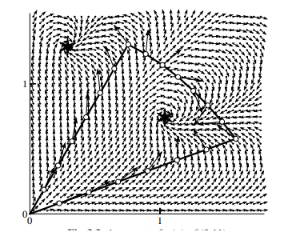
\includegraphics[width=0.5\linewidth]{images/arg_pz.png}
     \caption{Argument $p(z)$}
    Mỗi mũi tên tại điểm $z$ biểu diễn hướng của $\arg p(z)$ trên mặt phẳng phức; hai điểm được đánh dấu là các nghiệm của $p(z)$ (nguồn/đích của trường vector, tương ứng với điểm mà $\arg p(z)$ quay trọn một vòng xung quanh). Đường viền tam giác minh hoạ biên của quạt $S_j$ được xét trong chứng minh: cạnh đáy là tia $\arg z = 0$ (trục thực dương), hai cạnh còn lại là các tia biên $\arg z = 2\pi(j\mp \tfrac12)/k$. Có thể quan sát trực tiếp trên hình rằng nghiệm duy nhất của $p(z)$ nằm trong quạt $S_1$ nằm khá gần đĩa cấm $\{|z-1|\le 1\}$.
 \end{figure}
\noindent\textbf{Chặn trên cho phần dao động $I_1$}
Bước tiếp theo là chứng minh rằng nghiệm duy nhất nói trên, với $k$ đủ
lớn, thực sự rơi vào bên trong đĩa cấm $\{|z-1|\le 1\}$. Ta tách tích phân
\eqref{eq:bdf-p-integral} thành hai phần,
\[
p(z) = I_1 - I_2, \qquad
I_1 = \int_0^{r} \varphi(s)\,ds - e^{ik\theta}\int_0^{1} s^{k}\varphi(s)\,ds,
\qquad
I_2 = e^{ik\theta}\int_1^{r} s^{k}\varphi(s)\,ds,
\]
tức tách phần ứng với $s\le 1$ (dao động, bị chặn) khỏi phần ứng với
$s>1$ (tăng theo lũy thừa $s^k$).
 
Với hàm trọng $\varphi(s)$, ta có chặn
\[
|\varphi(s)| \le B(\theta), \qquad
B(\theta) = \begin{cases} |\sin\theta|^{-1}, & 0 < \theta \le \pi/2 \text{ hoặc } 3\pi/2 \le \theta < 2\pi,\\[2pt] 1, & \text{còn lại}. \end{cases}
\]
Ước lượng trực tiếp các tích phân trong $I_1$ (dùng chặn trên của
$\varphi$ và bất đẳng thức tam giác) dẫn tới
\begin{equation}
|I_1| \;\le\; \Bigl(r + \frac{1}{k+1}\Bigr) B(\theta)\;<\; r\,B(\theta)\,\frac{k+2}{k+1}, \qquad (r>1).\tag{3.2}\label{eq:3.2}
\end{equation}
 
\noindent\textbf{Chặn dưới cho phần tăng $I_2$}
 
Vì $s^{k}$ luôn dương trên đoạn lấy tích phân, ta có thể viết $I_2$ dưới
dạng
\[
I_2 = e^{ik\theta}\,\Phi \int_1^{r} s^{k}\,ds,
\qquad \Phi \in \text{bao lồi của } \{\varphi(s) : 1\le s\le r\}.
\]

Mọi phần tử của bao lồi này có thể viết dưới dạng
\[
\Phi = \alpha\,\varphi(s_1) + (1-\alpha)\,\varphi(s_2)
= \frac{\varphi(s_1)\,\varphi(s_2)}{\varphi(\hat s)},
\qquad 0\le\alpha\le 1,\ 1\le s_1,s_2\le r,
\]
với $\hat s = \alpha s_1 + (1-\alpha)s_2$. Do $|\varphi(s)|$ giảm đơn điệu theo $s$ khi $s\ge 1$, ta suy ra $|\Phi| \ge |\varphi(r)|$. Kết hợp với
$$\int_1^r s^k\,ds = (r^{k+1}-1)/(k+1)$$
ta được
\begin{equation}
|I_2| \;\ge\; \frac{r^{k+1}-1}{2r(k+1)} \;>\; \frac{r\bigl(r^{k-1}-1\bigr)}{2k+2}, \qquad (r>1).
\label{eq:bdf-I2-bound}
\end{equation}
 
\noindent\textbf{Kết hợp hai chặn và kết luận}
 
So sánh \eqref{eq:3.2} và \eqref{eq:3.3}, ta thấy rằng nếu
\begin{equation*}
r \;\ge\; R(\theta) := \Bigl( (2k+4)\,B(\theta) + 1 \Bigr)^{1/(k-1)}, \tag{3.3}\label{eq:3.3}
\end{equation*}
thì $|I_2| > |I_1|$, và do đó $p(z) = I_1 - I_2 \ne 0$ tại điểm
$z=re^{i\theta}$ đó. Nói cách khác, đường cong $r = R(\theta)$ cắt ra khỏi mỗi quạt $S_j$ một phần mà bên trong nó \emph{chắc chắn không} có nghiệm nào của $p(z)$ — phần còn lại giữa đường cong này và đĩa cấm $\{|z-1|\le 1\}$ chính là nơi duy nhất nghiệm của $p(z)$ trong quạt đó có thể có.
 
Với $k=12$, phần diện tích còn lại này đã đủ nhỏ để đảm bảo nghiệm duy
nhất trong quạt $S_1$ ($j\ne 0$) buộc phải nằm bên trong đĩa
$\{|z-1|\le 1\}$ — tức công thức BDF không ổn định tại $k=12$. Vì
$R(\theta)$ giảm đơn điệu theo $k$ với $\theta$ cố định (và điều tương tự đúng cho $R(\pi/k)$), điều này còn đúng cho mọi $k\ge 12$.
 
Với các giá trị trung gian $6 < k < 12$, tính không ổn định được xác nhận bằng tính toán số trực tiếp các nghiệm của $p(z)$.

\begin{figure}[H]
    \centering
    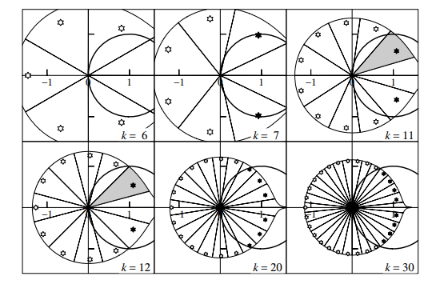
\includegraphics[width=0.85\textwidth]{images/root_pz.png}
    \caption{Phân bố các nghiệm của đa thức  $p_k(z)=\sum_{j=1}^{k}\frac{z^j}{j}$ trên mặt phẳng phức đối với một số giá trị của $k$. Đường tròn có tâm tại $(1,0)$ và bán kính $1$ biểu diễn miền $\{z:|z-1|<1\}$.
    Khi $k\le6$, mọi nghiệm đều nằm ngoài miền này; từ $k=7$ trở đi bắt đầu xuất hiện nghiệm nằm trong đĩa $|z-1|<1$, do đó điều kiện nghiệm của phương pháp BDF không còn được thỏa mãn.}
    \label{fig:roots-pk}
\end{figure}
Hình~\ref{fig:roots-pk} minh họa trực quan sự thay đổi vị trí các nghiệm của đa thức $p_k(z)$ khi số bước $k$ tăng. Có thể thấy rằng đối với $k=6$, toàn bộ các nghiệm vẫn nằm ngoài đĩa $|z-1|<1$, trong khi từ $k=7$ đã xuất hiện nghiệm đi vào miền này. Theo phép biến đổi Möbius, điều đó tương đương với việc đa thức đặc trưng của phương pháp BDF xuất hiện nghiệm có môđun lớn hơn $1$, làm vi phạm điều kiện 0-ổn định. Quan sát này phù hợp với kết quả của Định lý Dahlquist rằng họ phương pháp BDF chỉ 0-ổn định đối với $k\le6$.

Bảng tổng hợp kết quả về tính $0$-ổn định của các phương pháp BDF như sau.

\begin{table}[H]
\centering
\caption{Tính $0$-ổn định của các phương pháp BDF}
\label{tab:bdf-zero-stability}
\begin{tabular}{cc}
\hline
Bậc $k$ & Tính $0$-ổn định\\
\hline
$1\le k\le6$ & Có\\
$k\ge7$ & Không\\
\hline
\end{tabular}
\end{table}


\subsubsection{Kiểm chứng bằng số ranh giới $k \leq 6$}

Kết luận trên có thể được kiểm chứng trực tiếp bằng cách giải số phương trình
$\rho(z)=0$ cho từng giá trị $k$ và so sánh môđun lớn nhất trong các nghiệm với $1$.
Bảng~\ref{tab:bdf-stability} được sinh tự động từ mã nguồn đi kèm: với mỗi $k$, hệ số
của phương pháp BDF được dựng lại từ khai triển sai phân lùi
$\sum_{j=1}^{k}\frac{1}{j}\nabla^{j}Y_{n+k}=hf_{n+k}$, sau đó nghiệm của đa thức đặc
trưng thứ nhất được tính bằng phương pháp số.

\input{Sections/generated/bdf_stability}

Có thể thấy với mọi $k\le 6$, môđun lớn nhất đúng bằng $1$ và nghiệm đạt giá trị này
chính là nghiệm chính $z=1$ (nghiệm đơn), nên điều kiện nghiệm được thỏa mãn. Từ $k=7$,
môđun lớn nhất vượt ngưỡng ($1.0222$ khi $k=7$ và $1.1839$ khi $k=8$), phá vỡ điều kiện
nghiệm. Ranh giới $k\le 6$ vì vậy không phải là một quy ước được áp đặt, mà xuất hiện
như hệ quả trực tiếp từ vị trí nghiệm của đa thức đặc trưng.

\begin{figure}[H]
    \centering
    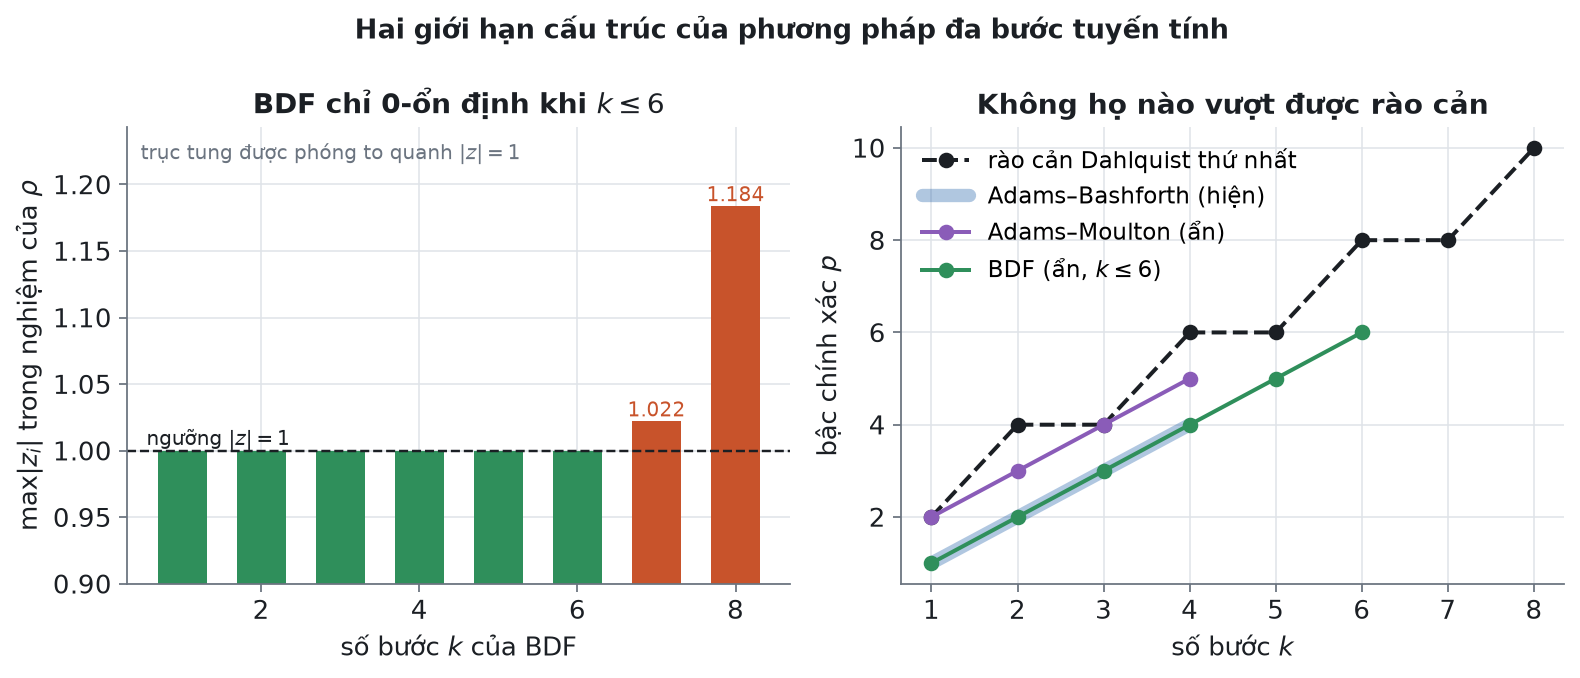
\includegraphics[width=\textwidth]{figures/fig06_dahlquist_barrier.png}
    \caption{Trái: môđun lớn nhất trong các nghiệm của $\rho(z)$ đối với họ BDF, trục
    tung được phóng to quanh ngưỡng $|z|=1$; các cột đỏ ($k=7,8$) vượt ngưỡng.
    Phải: bậc chính xác của ba họ phương pháp so với rào cản Dahlquist thứ nhất
    ($p\le k+2$ khi $k$ chẵn, $p\le k+1$ khi $k$ lẻ). Đường Adams--Bashforth được vẽ
    dày và mờ vì trùng hoàn toàn với đường BDF: cả hai đều có $p=k$.}
    \label{fig:dahlquist-barrier}
\end{figure}

\subsubsection{Miền ổn định tuyệt đối và bài toán cứng}

Tính $0$-ổn định là điều kiện khi $h\to 0$; trong tính toán thực tế, câu hỏi quan trọng
không kém là với một bước lưới $h$ \emph{cố định}, phương pháp chịu được những giá trị
$h\lambda$ nào. Miền ổn định tuyệt đối được xác định qua quỹ tích biên: ảnh của đường
tròn đơn vị dưới ánh xạ $z\mapsto \rho(z)/\sigma(z)$.

\begin{figure}[H]
    \centering
    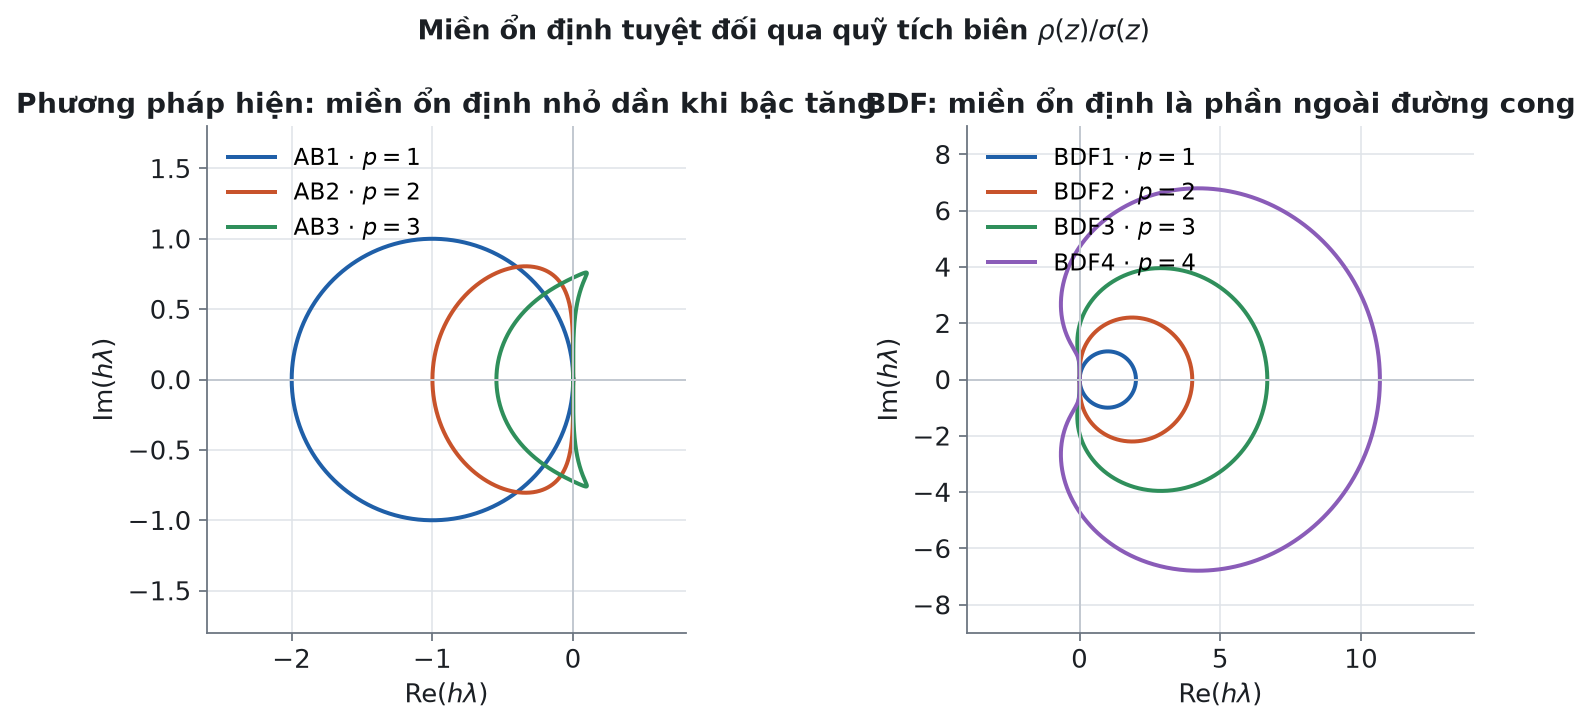
\includegraphics[width=\textwidth]{figures/fig05_stability_regions.png}
    \caption{Biên miền ổn định tuyệt đối. Với họ Adams--Bashforth (trái), miền ổn định
    nằm \emph{bên trong} đường cong và co lại nhanh khi bậc tăng: khoảng ổn định trên
    trục thực âm giảm từ $(-2,0)$ với AB1 xuống $(-6/11,0)\approx(-0.546,0)$ với AB3.
    Với họ BDF (phải), miền ổn định là phần \emph{bên ngoài} đường cong và chứa toàn bộ
    trục thực âm, nên bước lưới không bị ràng buộc bởi thành phần tắt dần nhanh.}
    \label{fig:stability-regions}
\end{figure}

Đây chính là lý do họ BDF được ưa dùng cho các bài toán cứng (stiff). Với bài toán
$y'=-1000\,(y-\cos t)-\sin t$, $y(0)=1$ và bước lưới $h=0.05$, ta có $h\lambda=-50$ nằm
ngoài miền ổn định của AB2 nên nghiệm số nổ tung, trong khi BDF2 vẫn cho sai số nhỏ hơn
$10^{-2}$. Cần nhấn mạnh rằng hai khái niệm là độc lập: AB2 vẫn $0$-ổn định và vẫn hội
tụ khi $h\to 0$, nhưng ở một bước lưới cụ thể thì hoàn toàn không dùng được.
